\subsection{Ligne de mise à feu}
\label{subsec:ligne_mise_a_feu}

La ligne de mise à feu est conçue pour assurer un allumage fiable et sécurisé du moteur du 2e étage de la fusée. Son objectif est
d'être capable de fournir assez de puissance à l'inflamateur lorsque le séquenceur donne l'odre de la mise à feu.

\begin{figure}[!h]
    \centering
    \begin{tabular}{rl}
        \begin{tabular}[b]{c}% if you add [t], than sub images are pushed down
            \begin{subfigure}{0.5\textwidth}
                \centering
                
\includegraphics[width=\textwidth]{figures/elec/PCB_Allumage_main.jpg}
                \caption{(principale, côté composants)}
            \end{subfigure}\\
            \begin{subfigure}{0.5\textwidth}
                \centering
                
\includegraphics[width=\textwidth]{figures/elec/PCB_Allumage_main_back.jpg}
                \caption{(principale, côté interface)}
            \end{subfigure}
        \end{tabular}
        &
        \begin{subfigure}{0.4\textwidth}
            \centering
            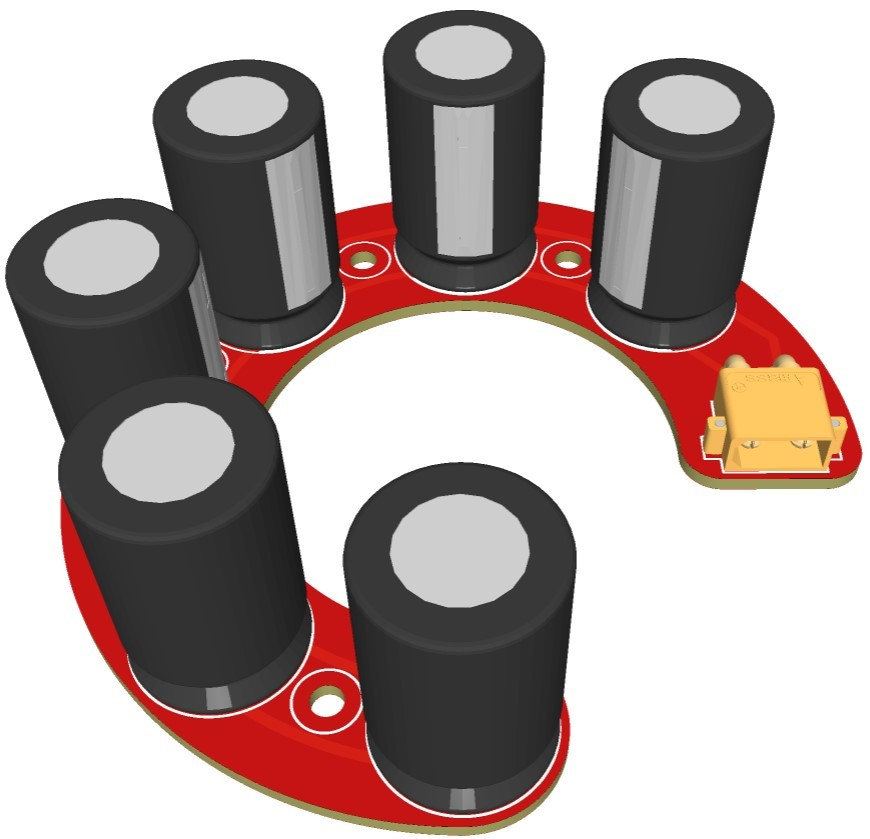
\includegraphics[width=\textwidth]{figures/elec/PCB_Allumage_Condo_2.jpg}
            \caption{(condensateurs)}
        \end{subfigure}
    \end{tabular}
    \caption{Rendu 3D des cartes PCBs principale et condensateurs dy système d'allumage}
\end{figure}

\subsubsection{Principe de fonctionnement}

\begin{minipage}{0.55\textwidth}
    Le système repose sur une alimentation constituée d’une batterie Li-Po de faible puissance associée à un réhausseur de
    tension, permettant la charge d’une banque de condensateurs (déportée de la carte d’allumage principale) à travers une
    résistance, sur une durée courte.\\

    Une fois le système armé, cette banque de condensateurs est connectée à deux transistors \acrshort{MOSFET} normalement
    bloquants. L’ordre de mise à feu est transmis par le séquenceur sous forme d’une impulsion commandant deux optocoupleurs,
    lesquels pilotent l’ouverture des \acrshort{MOSFET}. Ceux-ci deviennent alors conducteurs et autorisent le passage du
    courant.\\

    Deux shunts de sécurité, réalisés sous forme de courts-circuits, peuvent être insérés afin d’assurer une protection
    pyrotechnique. En leur absence, un buzzer est activé et la ligne pyrotechnique reliée à l’inflammateur du moteur du second
    étage est mise sous tension.
\end{minipage}
\hfill
\begin{minipage}{0.40\textwidth}
    \begin{figure}[H]
        \centering
        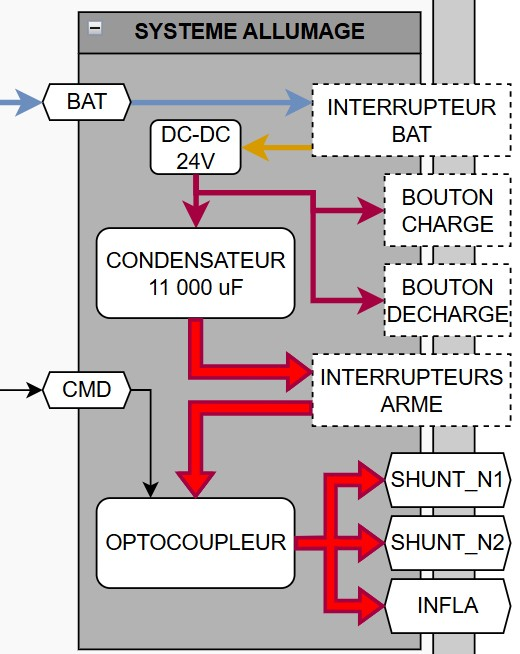
\includegraphics[width=\textwidth]{figures/elec/syno_allumage.jpg}
        \caption{Zoom sur le sinopsis de la ligne de mise à feu (ref. annexe \ref{subsec:synoptique_fusee})}
    \end{figure}
\end{minipage}

\newpage

La banque de condensateurs, directement connectée à cette ligne de faible impédance, est alors capable de délivrer un courant
élevé, suffisant pour activer l'inflammateur et initier la combustion du moteur du deuxième étage.

\begin{figure}[h!]
    \centering
    
\includegraphics[width=\textwidth]{figures/elec/Syno_Allumage_2.jpg}
    \caption{Schéma de la ligne de mise à feu}
    \label{fig:schema_allumage}
\end{figure}

Le schema ci-haut (figure \ref{fig:schema_allumage}) présente une autre vision de la ligne de mise à feu.

\paragraph*{Circuit de charge/décharge des condensateurs}

Le circuit de charge/décharge des condensateurs est conçu pour assurer une charge et une décharge contrôlées de la banque de
condensateur à l'aide de résistances évitant les courants d'appel élevés qui pourraient endommager les composants ou présenter un
danger pour les opérateurs.

\begin{figure}[h!]
    \centering
    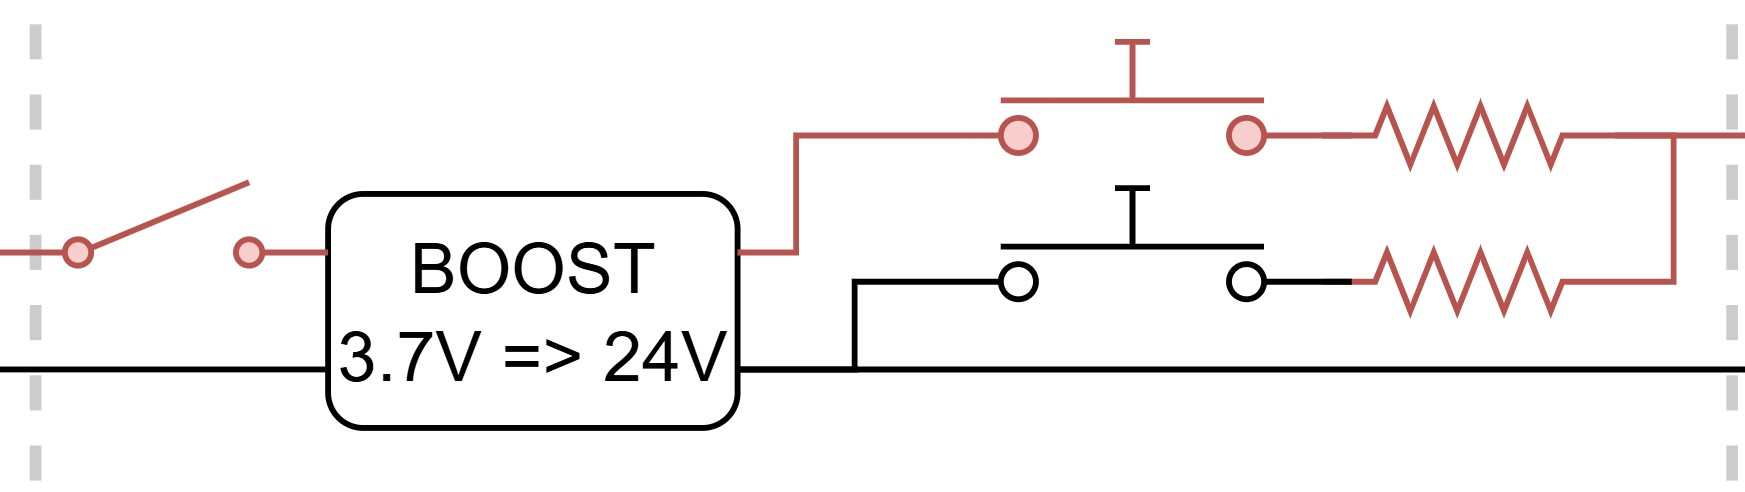
\includegraphics[width=0.55\textwidth]{figures/elec/Syno_allumage_charge.jpg}
    \caption{Zoom sur le circuit de charge/décharge des condensateurs}
    \label{fig:schema_allumage_charge}
\end{figure}

Il se compose en premier lieu d'un interrupteur batterie qui permet d'alimenter ou de couper l'alimentation de la ligne de mise à
feu. Lorsque l'interrupteur est fermé, une led rouge s'allume. La batterie alimente un circuit réhausseur de tension passant de
3.7V à 24V et basé sur le composants MSKSEMI-MSDB628. Cela permet d'augmenter la densité énergétique stockée dans les
condensateurs. Ensuite, deux boutons poussoir autobloquant nommé "charge" et "décharge" permet connecter la banque de
condensateurs soit au 24V, soit à la masse et ce au travers d'une résistance de 402 $\Omega$. Le courant maximal de charge ou de
décharge est alors de :

$$I = \frac{V}{R} = \frac{24V}{402\Omega} \approx 60mA$$

\paragraph*{Circuit condensateurs}

Le circuit de condensateurs est conçu pour stocker l'énergie nécessaire à l'allumage du moteur du deuxième étage et pour la
délivrer suffisamment rapidement lorsque le séquenceur donne l'ordre de mise à feu.

\begin{figure}[h!]
    \centering
    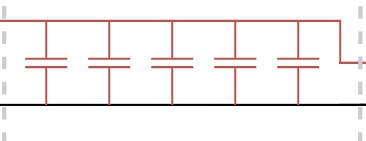
\includegraphics[width=0.5\textwidth]{figures/elec/Syno_Allumage_Condo.jpg}
    \caption{Zoom sur le circuit de condensateurs}
    \label{fig:schema_allumage_condensateurs}
\end{figure}

Il se compose d'une banque de 6 condensateurs électrolytiques de 4700 $\mu$F chacun, connectés en parallèle, ce qui donne une
capacité totale de 28.2 mF.

\newpage

Il est écrit dans le \acrlong{CDC} :

\begin{quote}
    (Règle) \textit{INF1 : Pour détoner, l’inflammateur doit être alimenté par un courant de 4A pendant 30ms.
    Sa résistance interne (tant qu’il n’a pas détoné) est de 1$\Omega$.}\newline\cite[p.~73]{CDC_BiEtage}
\end{quote}

La cinématique de décharge des condensateurs est donnée par la formule suivante :

\begin{align*}
    I(t) &= \frac{V_{max}}{R} e^{-\frac{t}{RC}} \\
    &= \frac{24}{1} e^{-\frac{t}{1\times0.0282}} \\
    &\approx 24e^{-\frac{t}{0.0282}}
\end{align*}

Vu que la fonction est bijective, on peut également déterminer la fonction inverse qui nous donne l'instant à laquel le courant
atteint une valeur donnée :

\begin{align*}
    I &= \frac{V_{max}}{R} e^{-\frac{t(I)}{RC}} \\
    \frac{RI}{V_{max}} &= e^{-\frac{t(I)}{RC}} \\
    \ln{\left(\frac{V_{max}}{RI}\right)} &= -\frac{t(I)}{RC} \\
    t(I) &= RC\ln{\left(\frac{V_{max}}{RI}\right)} \\
    t(I) &= 0.0282 \times \ln{\left(\frac{24}{I}\right)}
\end{align*}

Cela nous permet de trouver l'instant tel que système se trouve en dessous des 4 A : $t(4) = 50.52\ ms$. Nous sommes donc
bien au dessus des 30 ms requis pour l'allumage de l'inflammateur. Nous pouvons également calculer le delta de courant entre
ce que le cahier des charges demande et ce que le système délivre à l'instant de 30 ms : $I(0.03) = 8.283\ A$. Nous avons donc une
marge de 4.283 A à l'instant de 30 ms, ce qui est largement suffisant pour assurer un allumage fiable du moteur du deuxième étage.\\

On estime le temps de charge complet théorique de la banque de condensateurs à 5 fois la constante de temps, soit :
$5\tau = 5\times RC = 5 \times 402 \times 0.0282 = 5 \times 11.3364 = 56.682\ s$

\newpage

\paragraph*{Circuit isolateur}

Le circuit isolateur est conçu pour assurer une isolation galvanique entre la ligne de mise à feu et les autres éléments du
système électronique de la fusée tout en permettant la transmission du signal de mise à feu du séquenceur au circuit d'allumage.

\begin{minipage}{0.45\textwidth}
    Il se compose tout d'abord de deux interrupteurs correspondant aux interrupteur des pyrotechniciens.\\

    Puis, deux optocoupleurs et de deux transistors \acrshort{MOSFET} jouant le rôle respectivement de commutateur à haut
    potentiel et de commutateur à bas potentiel, l'un étant sur la ligne positive et l'autre sur la ligne neutre.\\
    
    Lorsque le séquenceur donne l'ordre de mise à feu, il envoie une impulsion qui active les optocoupleurs. Ceux-ci pilotent
    l'ouverture des \acrshort{MOSFET} qui deviennent alors conducteurs et permettent le passage du courant de la banque de
    condensateurs vers l'inflammateur du moteur du deuxième étage.
\end{minipage}
\hfill
\begin{minipage}{0.45\textwidth}
    \begin{figure}[H]
        \centering
        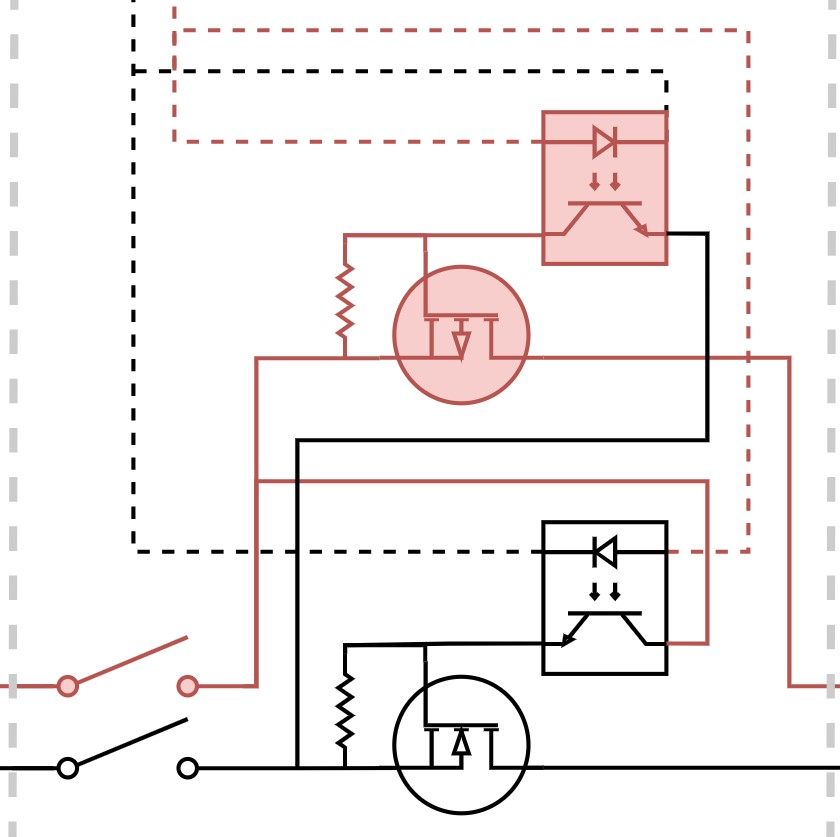
\includegraphics[width=\textwidth]{figures/elec/Syno_Alumage_Iso.jpg}
        \caption{Zoom sur le circuit isolateur}
        \label{fig:schema_allumage_isolateur}
    \end{figure}
\end{minipage}

\paragraph*{Circuit final}

La fin du circuit comporte un buzzer, deux shunts et une résistance à relativement haute impédence.\\

\begin{minipage}{0.4\textwidth}
    \begin{figure}[H]
        \centering
        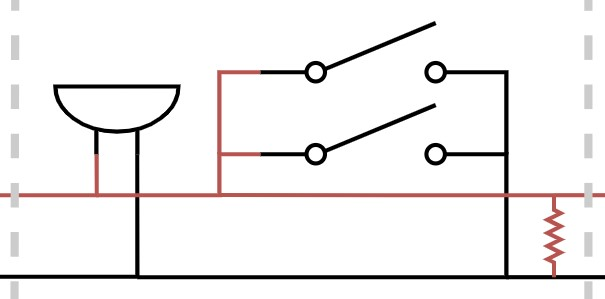
\includegraphics[width=\textwidth]{figures/elec/Syno_Allumage_end.jpg}
        \caption{Zoom sur le circuit final}
        \label{fig:schema_allumage_final}
    \end{figure}
\end{minipage}
\hfill
\begin{minipage}{0.55\textwidth}
    Le buzzer joue le rôle d'indicateur sonore indiquant que la ligne pyrotechnique est sous tension.\\

    Les deux shunts sont des sécurités supplémentaires faisant court-circuit au cas où un courant est présent alors que les
    conditions d'allumage ne sont pas réuni. En pratique, qu'un seul des deux shunts sera utilisé et sera attaché à la rampe de
    la fusée rendat ainsi les opérations aux sols plus sûr. \\

    La résistance permet au système de se déchargé une fois l'inflammateur utilisé.
\end{minipage}

\subsubsection{Interface}

\begin{minipage}{0.55\textwidth}
    L'interface du système d'allumage se compose de 3 interrupteurs, de 2 boutons autobloquant et de 6 LEDs.\\

    Parmi les 3 interrupteurs, le premier (le plus haut) est nommé interrupteur \verb|BAT|. Il connecte ou déconnecte la batterie
    au système. Lorsque la batterie est connecté, la led nommé \verb|BAT| s'illumine en rouge.\\
    
    Les deux autres inerrupteurs correspondent aux interrupteurs pyrotechique. Ils connectent (respectivement de haut en bas) le 
    haut potentielle (\verb|VCC|) et le bas potentiel (\verb|GND|) des condensateurs aux \acrshort{MOSFET} de blocage. La led
    \verb|ARME| indique le niveau de tension entre les deux \acrshort{MOSFET} entre 0 et 24 V.\\
\end{minipage}
\hfill
\begin{minipage}{0.4\textwidth}
    \begin{figure}[H]
        \centering
        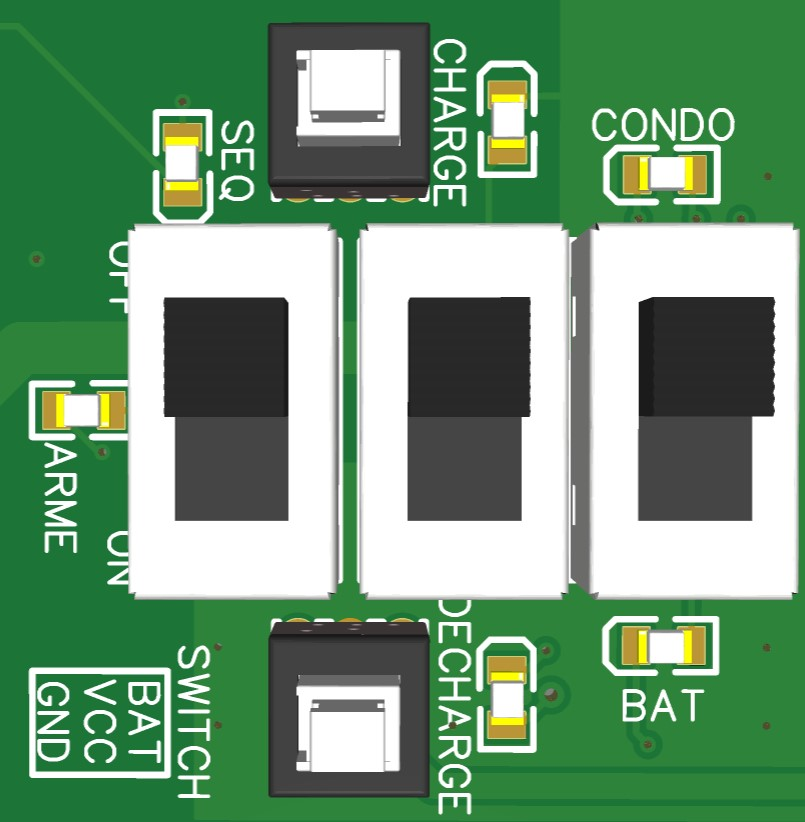
\includegraphics[width=0.9\textwidth, angle=90]{figures/elec/PCB_Alumage_main_interface.jpg}
        \caption{Zoom sur l'interface de la carte principale du système d'allumage}
    \end{figure}
\end{minipage}

\vspace{0.2cm}

Le bouton de gauche (nommé \verb|CHARGE|) permet de charger les condensateurs tandi que le bouton de droite (nommé
\verb|DECHARGE|) permet de les décharger. Pour les deux boutons, lorsque l'un d'entre eux est enfoncé, une led située juste
au dessus de lui s'illumine en bleu indiquant l'état courant de charge ou de décharge. A noté que le fait de charger et décharger
les condensateurs en même temps a pour effet potentiel de placer les condensateurs dans un état indéterminé mais non dangereux.\\

La led nommée \verb|CONDO| indique l'état de charge des condensateurs entre 0 et 24 V.\\

La led nommée \verb|SEQ| indique l'état du signal électrique venant du séquenceur et commendant l'état ouvert ou fermé des
\acrshort{MOSFET}.\\

A noté que toutes les led sont directement allimenté par la batterie et non pas les condensateurs, permettant ainsi de maximiser
l'énergie présent dans la banque de condensateur avant libération d'énergie dans l'inflamateur.

\subsubsection{Séquence de vol}

Voici la chronologie des événements attendu concernant la ligne de mise à feu :

\begin{enumerate}
    \item Vérifier la présence du shunt de sécurité et de son bon état. 
    \item Vérifier l'état de tous les interrupteurs: \verb|OFF|.
    \item Vérifier l'état de toutes les LEDs: éteint.
    \item Changer l'état de l'interrupteur \verb|BAT| à \verb|ON|.
    \item Vérifier que la led \verb|BAT| s'allume en \textcolor{red}{rouge} et que les autres LEDs restent éteintes.
    \item Si la les \verb|DECHARGE| s'allume en \textcolor{blue}{bleu}, changer l'état du bouton \verb|DECHARGE| à \verb|OFF|.
\end{enumerate}
A cette étape, le système est prêt à être charger en énergie.
\begin{enumerate}[resume]
    \item Changer l'état du bouton \verb|CHARGE| à \verb|ON|.
    \item Vérifier que la led \verb|CHARGE| s'allume en \textcolor{blue}{bleu}.
    \item Attendre 1 minute pour que les condensateurs soient complètement chargé.
    \item Vérifier que la led \verb|CONDO| soit allumée en \textcolor{red}{rouge}.
    \item Vérifier que la led \verb|SEQ| soit éteinte et que le buzzer soit éteint.
\end{enumerate}
A cette étape, le système est prêt à être armé.
\begin{enumerate}[resume]
    \item Changer l'état de l'interrupteur \verb|VCC| à \verb|ON|.
    \item Changer l'état de l'interrupteur \verb|GND| à \verb|ON|.
    \item Vérifier que la led \verb|ARME| s'allume en \textcolor{green}{vert}.
    \item Vérifier que la led \verb|CHARGE| est toujours allumée en \textcolor{blue}{bleu}.
\end{enumerate}
A cette étape, le système est armé et prêt à être mis à feu. C'est l'état final du système avant le lancement de la fusée.\\

Lorsque le séquenceur donne l'ordre de mise à feu, la led \verb|SEQ| s'allume en \textcolor{red}{rouge}. Le buzzer se met
également en route tant qu'il y a du courant dans les condensateurs et que les shunts de sécurité ne sont pas en place.

\newpage
